Un Turno como explicamos con anterioridad representa en las unidades que dividimos un Partido para que este se desarolle. De esta forma al intentar modelar los turnos vimos que un turno debia conocer dos equipos, uno como el equipo que comienza con la pelota, es decir comienza atacando, y otro que comienza sin la pelota. Ademas decidimos que el turno es el responsable de pedirle a cada Equipo su jugada pertinente (ofensivo o defensiva) y el responsable de ir comunicado a ambas jugadas.
Por otro lado, notamos que la accion de Reboteo era algo ajeno a las jugadas, por lo tanto el turno en si es el que usa esta acción y no las jugadas.
Al igual que Partido, el Turno tambien conoce un Logger para poder dejar registro de las acciones que van sucediendo.
De esta forma llegamos al siguiente diagrama de clases:

\begin{center}
  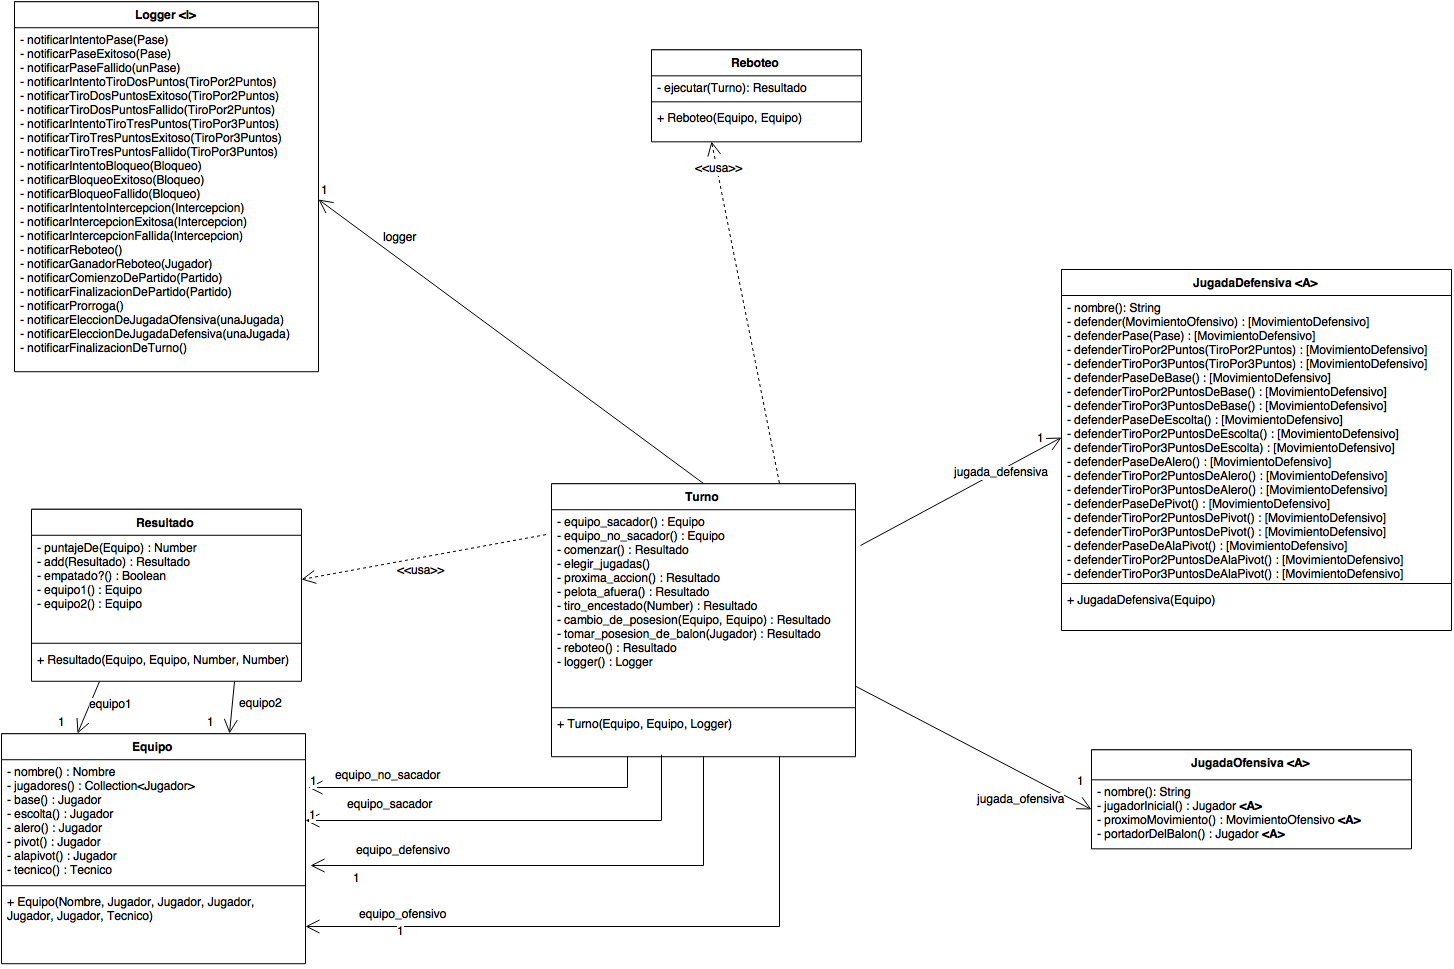
\includegraphics[scale=0.35]{imagenes/clases-turno.png}
\end{center}

Como dijimos entonces, el turno es el responsable de instancias las Jugadas de cada equipo y controlar sus ejuciones y comunicarlas entre si, pero es resposablidad de las acciones (pase, tiro, intercepcion, etc) en si, notificarle al turno como seguir (es decir si tuvieron exito o no), para esto el turno sabe response mensajes del estilo, proxima_accion, pelota_afuera, tiro_encestado, etc. De esta forma El turno se entera que debe hacer a continuacion y luego al finalizar el turno, sea por un balon encestado o un balon afuera, se crea el resultado correcto y se empieza a devolver este resultado hasta llegar al turno de nuevo y este lo devuelve para arriba.
De esta forma el turno no conoce de como resolver las acciones en particular. Pero si resuelve que se hace en caso de exito o falla de ellas. Por ejemplo, en caso de concretarse una intercepción, el turno es el que hace que se cambie la posesion, el equipo atacante pasa a ser defensivo y el defensivo pasa a ser atacante, se vuelve a elegir jugadas y se ponen en marcha estas nuevas jugadas.

A continuación presentamos un par de diagramas de secuencias para explicar el funcionamiento basico del metodo comenzar: \\

En el primer diagrama de secuencia representamos el escenario de un turno donde la Jugada Ofensiva elegida es de 1 pase y luego un tiro de tres puntos y la jugada defensiva es hombre a hombre. En particular el pase no es interceptado y llega con exito y el tiro no es bloqueado y es entra exitosamente al aro, por lo que el resultado que terminar devolviendo el turno es de 3 a 0.
\begin{center}
  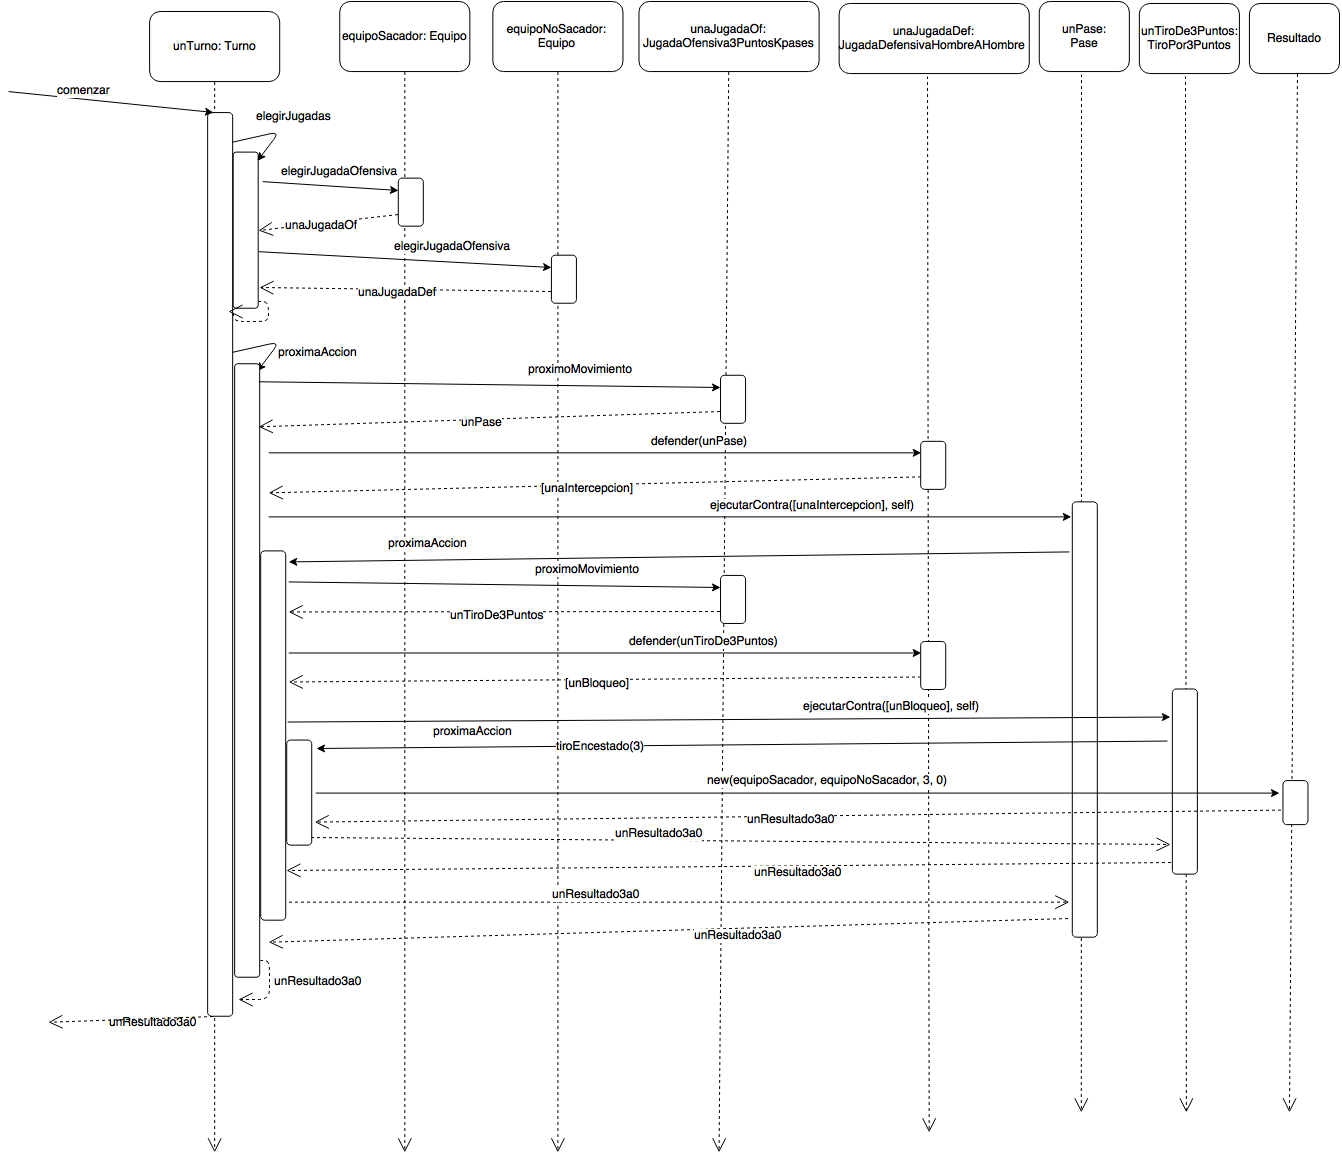
\includegraphics[scale=0.35]{imagenes/turno-pase-y-tiro-exitosos.png}
\end{center}

En el proximo diagrama mostramos un escenario donde la jugada ofensiva elegida es de 3 pases y tiro de 3 puntos y la jugada defensiva es hombre a hombre. Pero en este caso el primer pase no es interceptado pero es errado, por lo que la pelota se va fuera de la cancha, finalizando el turno con un resultado de 0 a 0.
\begin{center}
  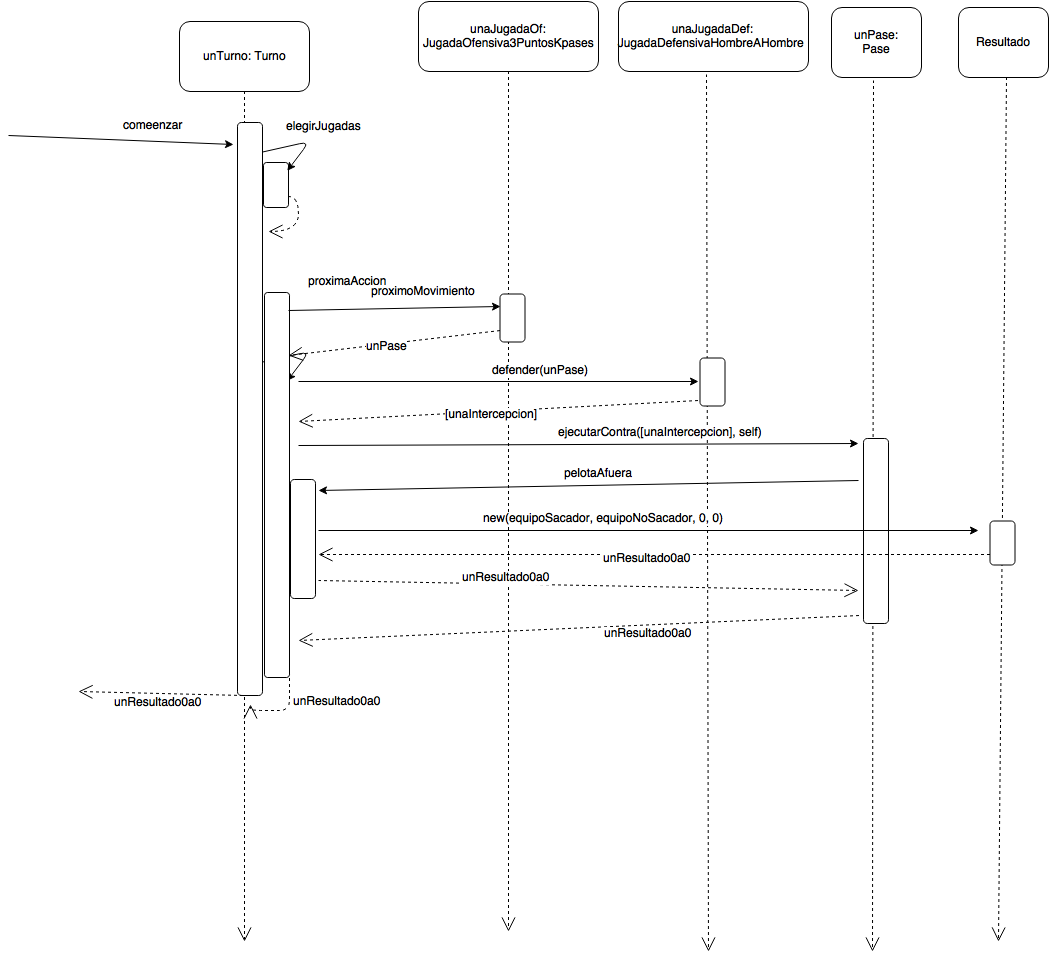
\includegraphics[scale=0.45]{imagenes/turno-pase-afuera.png}
\end{center}
